% 本模板根据中国科学院大学本科生公共必修课程《基础物理实验》Word模板格式编写
% 本模板由Shing-Ho Lin和Jun-Xiong Ji于2022年9月共同完成, 旨在方便LaTeX原教旨主义者和被Word迫害者写实验报告, 避免Word文档因插入过多图与公式造成卡顿. 
% 如有任何问题, 请联系: linchenghao21@mails.ucas.ac.cn
% This is the LaTeX template for experiment report of Experimental Physics courses, based on its provided Word template. 
% This template is completed by the joint collabration of Shing-Ho Lin and Junxiong Ji in September 2022. 
% Adding numerous pictures and equations leads to unsatisfying experience in Word. Therefore LaTeX is better. 
% Feel free to contact us via: linchenghao21@mails.ucas.ac.cn

\documentclass[11pt]{article}

\usepackage[a4paper]{geometry}
\geometry{left=2.0cm,right=2.0cm,top=2.2cm,bottom=2.2cm}

\usepackage{ctex} % 支持中文的LaTeX宏包
\usepackage{amsmath,amsfonts,graphicx,subfigure,amssymb,bm,amsthm,mathrsfs,mathtools,breqn} % 数学公式和符号的宏包集合
\usepackage{algorithm,algorithmicx} % 算法和伪代码的宏包
\usepackage[noend]{algpseudocode} % 算法和伪代码的宏包
\usepackage{fancyhdr} % 自定义页眉页脚的宏包
\usepackage[framemethod=TikZ]{mdframed} % 创建带边框的框架的宏包
\usepackage{fontspec} % 字体设置的宏包
\usepackage{adjustbox} % 调整盒子大小的宏包
\usepackage{fontsize} % 设置字体大小的宏包
\usepackage{tikz,xcolor} % 绘制图形和使用颜色的宏包
\usepackage{multicol} % 多栏排版的宏包
\usepackage{multirow} % 表格中合并单元格的宏包
\usepackage{pdfpages} % 插入PDF文件的宏包
\RequirePackage{listings} % 在文档中插入源代码的宏包
\RequirePackage{xcolor} % 定义和使用颜色的宏包
\usepackage{wrapfig} % 文字绕排图片的宏包
\usepackage{bigstrut,multirow,rotating} % 支持在表格中使用特殊命令的宏包
\usepackage{booktabs} % 创建美观的表格的宏包
\usepackage{circuitikz} % 绘制电路图的宏包
\usepackage[inline]{enumitem}
\usepackage{tabularx}

\usepackage{indentfirst}
\setlength{\parindent}{2em}
\setlength{\abovecaptionskip}{2pt}
\setlength{\belowcaptionskip}{2pt}
\setlength{\intextsep}{8pt}
\setlength{\floatsep}{8pt}

\definecolor{dkgreen}{rgb}{0,0.6,0}
\definecolor{gray}{rgb}{0.5,0.5,0.5}
\definecolor{mauve}{rgb}{0.58,0,0.82}
\lstset{
  frame=tb,
  aboveskip=3mm,
  belowskip=3mm,
  showstringspaces=false,
  columns=flexible,
  framerule=1pt,
  rulecolor=\color{gray!35},
  backgroundcolor=\color{gray!5},
  basicstyle={\small\ttfamily},
  numbers=none,
  numberstyle=\tiny\color{gray},
  keywordstyle=\color{blue},
  commentstyle=\color{dkgreen},
  stringstyle=\color{mauve},
  breaklines=true,
  breakatwhitespace=true,
  tabsize=3,
}

% 轻松引用, 可以用\cref{}指令直接引用, 自动加前缀. 
% 例: 图片label为fig:1
% \cref{fig:1} => Figure.1
% \ref{fig:1}  => 1
\usepackage[capitalize]{cleveref}
% \crefname{section}{Sec.}{Secs.}
\Crefname{section}{Section}{Sections}
\Crefname{table}{Table}{Tables}
\crefname{table}{Table.}{Tabs.}

\setmainfont{Palatino Linotype.ttf}
\setCJKmainfont{SimHei.ttf}
% \setCJKsansfont{Songti.ttf}
% \setCJKmonofont{SimSun.ttf}
\punctstyle{kaiming}
% 偏好的几个字体, 可以根据需要自行加入字体ttf文件并调用

\renewcommand{\emph}[1]{\begin{kaishu}#1\end{kaishu}}

%改这里可以修改实验报告表头的信息
\newcommand{\experiName}{微波布拉格衍射}
\newcommand{\supervisor}{耿直}
\newcommand{\name}{张欣培}
\newcommand{\studentNum}{2022K8009922001}
\newcommand{\class}{01}
\newcommand{\group}{10}
\newcommand{\seat}{4}
\newcommand{\dateYear}{2023}
\newcommand{\dateMonth}{11}
\newcommand{\dateDay}{20}
\newcommand{\room}{教715}
\newcommand{\others}{$\square$}
%% 如果是调课、补课, 改为: $\square$\hspace{-1em}$\surd$
%% 否则, 请用: $\square$
%%%%%%%%%%%%%%%%%%%%%%%%%%%

\begin{document}

%若需在页眉部分加入内容, 可以在这里输入
% \pagestyle{fancy}
% \lhead{\kaishu 测试}
% \chead{}
% \rhead{}

\begin{center}
    \LARGE \bf 《\, 基\, 础\, 物\, 理\, 实\, 验\, 》\, 实\, 验\, 报\, 告
\end{center}

\begin{center}
    \noindent \emph{实验名称}\underline{\makebox[25em][c]{\experiName}}
    \emph{指导教师}\underline{\makebox[8em][c]{\supervisor}}\\
    \emph{姓名}\underline{\makebox[6em][c]{\name}} 
    % 如果名字比较长, 可以修改box的长度"6em"
    \emph{学号}\underline{\makebox[10em][c]{\studentNum}}
    \emph{分班分组及座号} \underline{\makebox[5em][c]{\class \ -\ \group \ -\ \seat }\emph{号}} (\emph{例}:\, 1\,-\,04\,-\,5\emph{号})\\
    \emph{实验日期} \underline{\makebox[3em][c]{\dateYear}}\emph{年}
    \underline{\makebox[2em][c]{\dateMonth}}\emph{月}
    \underline{\makebox[2em][c]{\dateDay}}\emph{日}
    \emph{实验地点}\underline{{\makebox[4em][c]\room}}
    \emph{调课/补课} \underline{\makebox[3em][c]{\others\ 是}}
    \emph{成绩评定} \underline{\hspace{5em}}
    {\noindent}
    \rule[8pt]{17cm}{0.2em}
\end{center}


\begin{center}
    \Large \bf 第一部分\qquad 实验内容
\end{center}

\section{实验预习报告}
\begin{figure}[H]
    \centering
    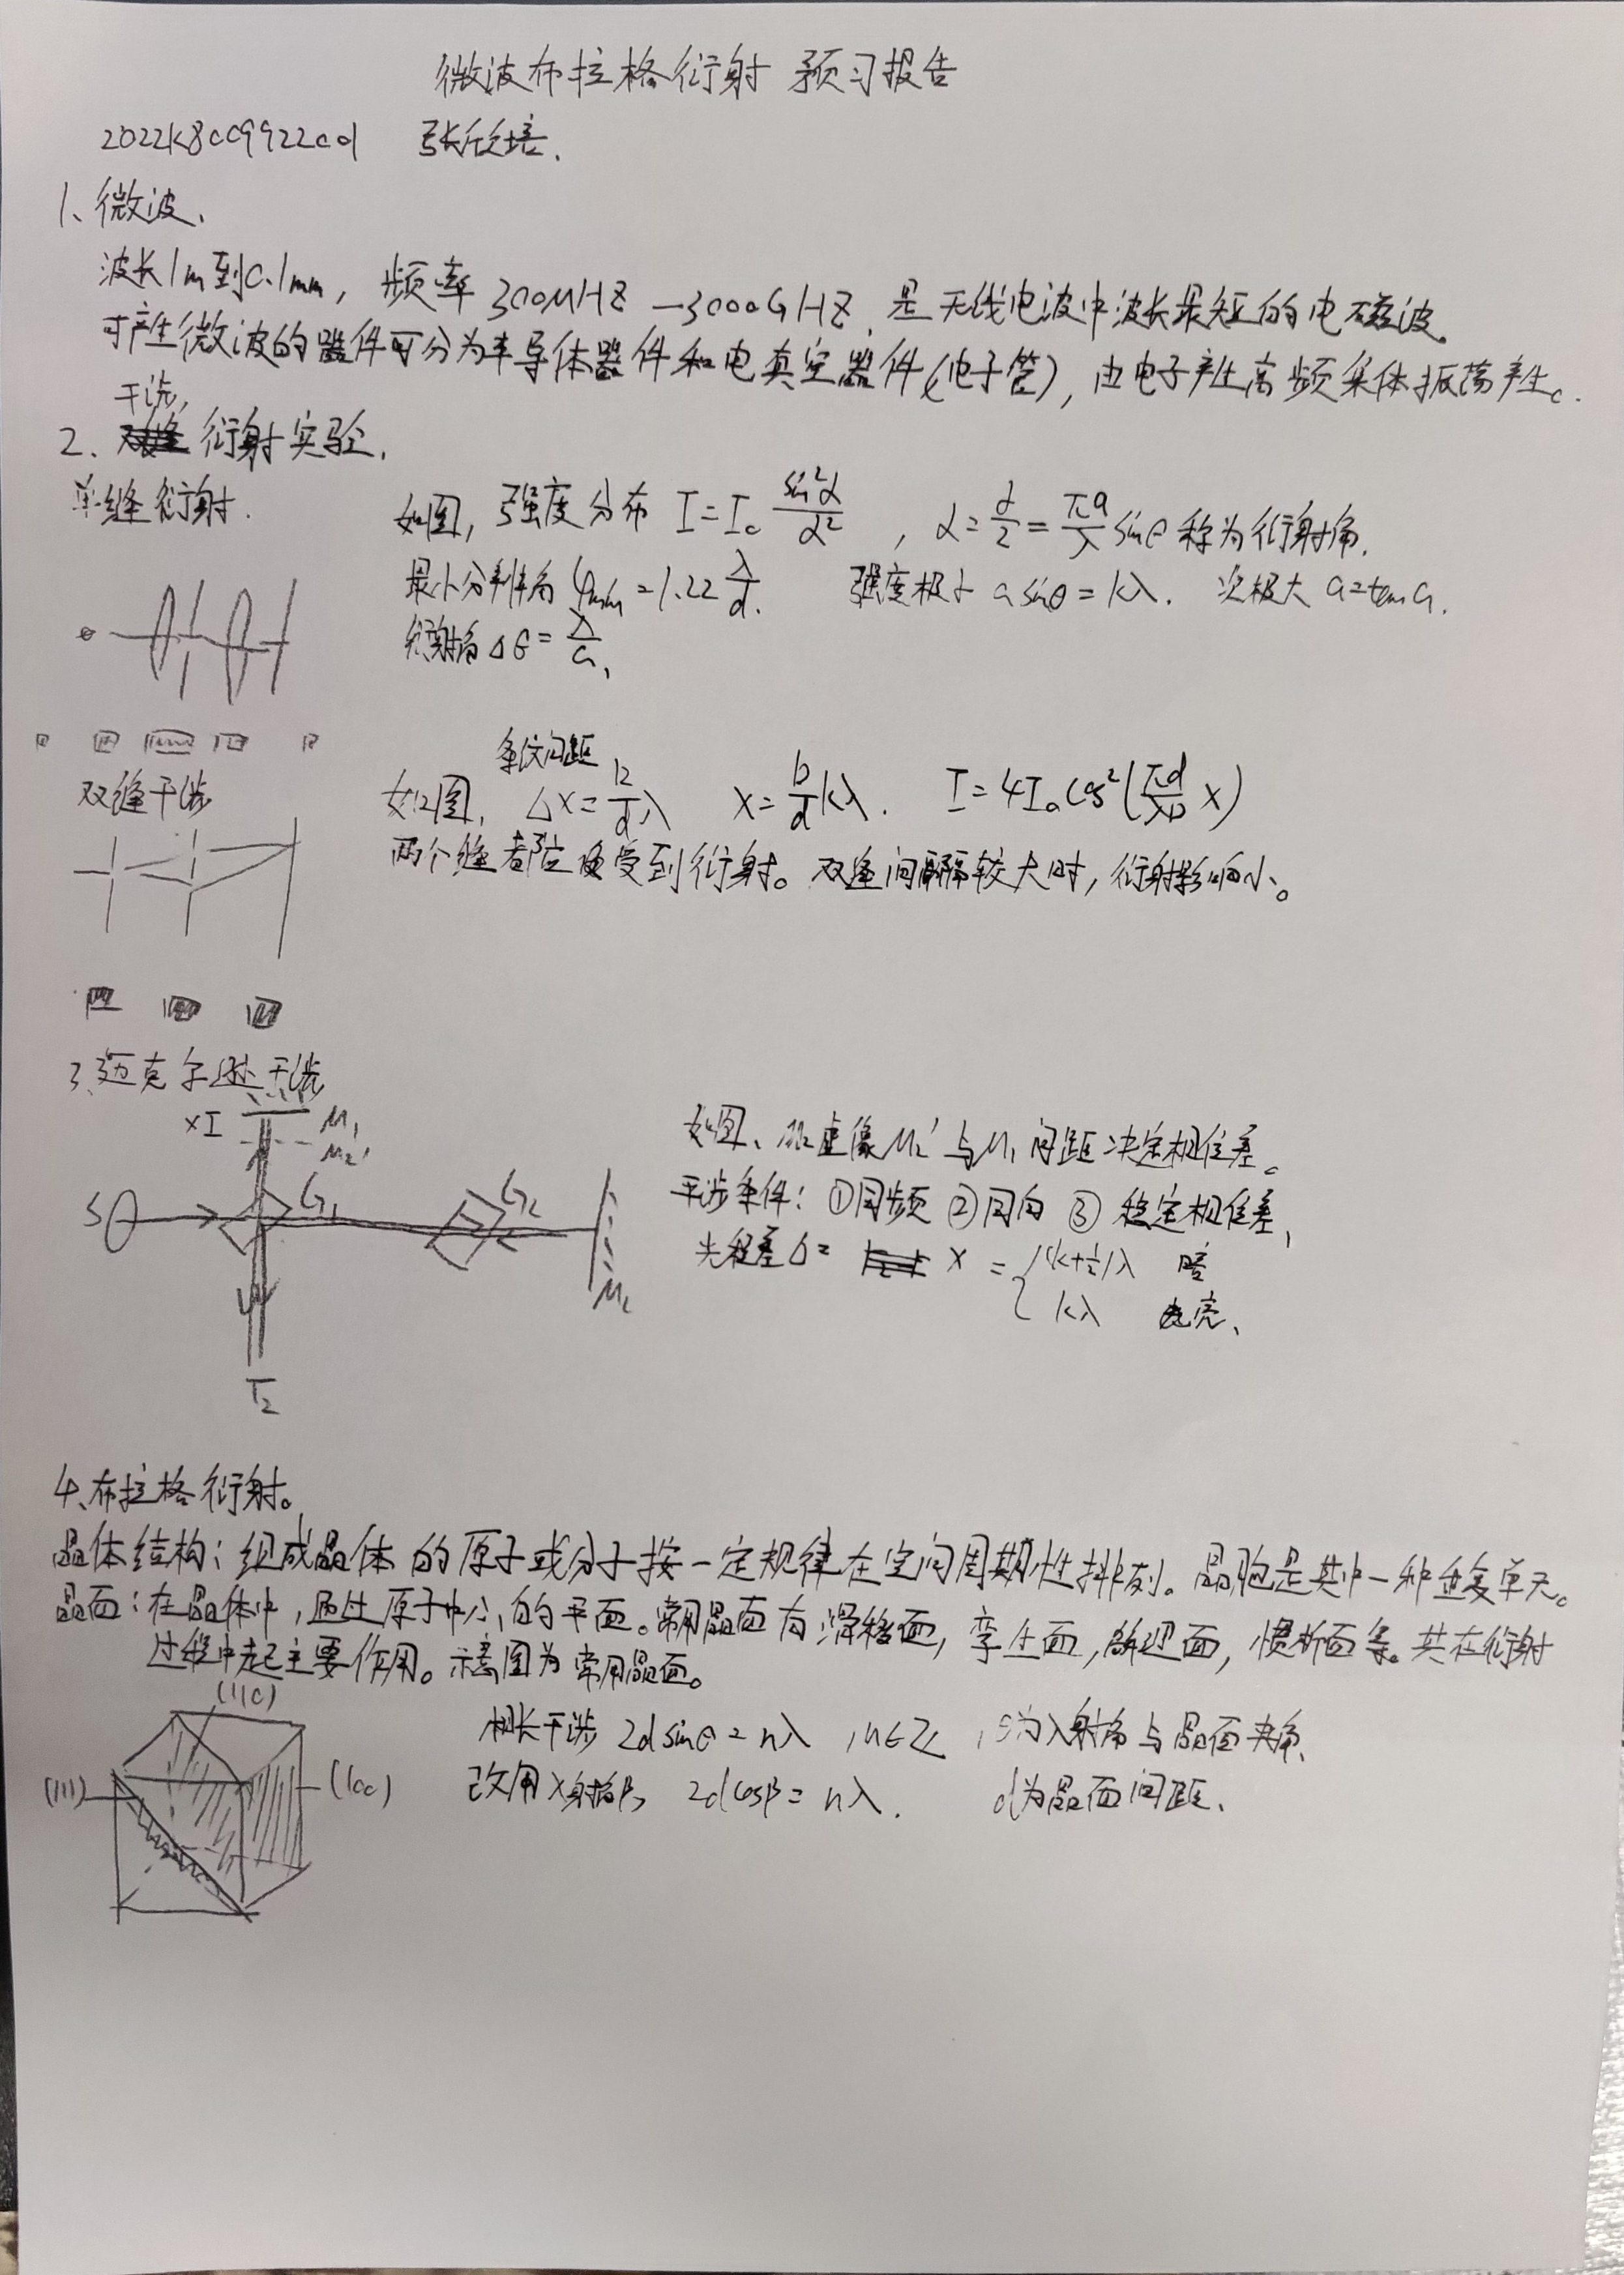
\includegraphics[width=13.5cm]{Fig/1.jpg}
\end{figure}

\section{实验目的}
\begin{enumerate}
    \item 了解与学习微波产生的基本原理以及传播和接收等基本特性。
    \item 观测微波双缝衍射、单缝干涉等实验现象。
    \item 观测模拟晶体的微波布拉格衍射现象。
    \item 通过迈克耳逊实验测量微波波长。
\end{enumerate}

\section{实验器材}

    \par \indent DHMS-1型微波光学综合实验仪一套,包括 X波段微波信号源、微波发生器、发
    射喇叭、接收喇叭、微波检波器、检波信号数字显示器、可旋转载物平台和支架,以及实验用附
    件(反射板、分束板、单缝板、双缝板、模拟晶体模型 、读数机构等)。
    \begin{figure}[H]
        \centering
        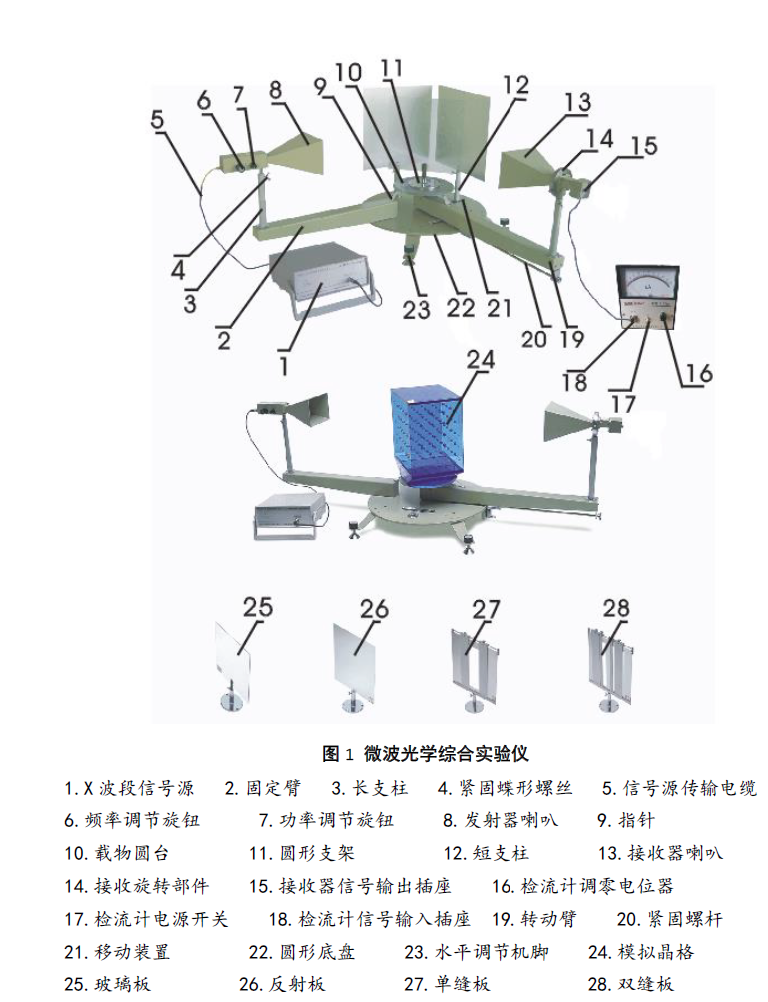
\includegraphics[width=10cm]{Fig/2.png}
        \caption{DHMS-1型微波光学综合实验仪}
    \end{figure}

\section{实验原理}
\begin{enumerate}[itemjoin=\\]
    \item 微波的产生和接收
    \par \hspace*{2em} 本实验使用的微波发生器是
    采用电调制方法实现的,优点是应用灵活,参数调配方便,适
    用于多种微波实验 ,其工作原理框图见图 2。微波发生器内部有一个电压可调控制的 VCO,用于
    产生一个 4.4GHz-5.2GHz的信号,它的输出频率可以随输入电压的不同作相应改变,经过滤波
    器后取二次谐波 8.8GHz-9.8GHz,经过衰减器作适当的衰减后,再放大,经过隔离器后,通过探
    针输出至波导口,再通过E 面天线发射出去。接收部分采用检波/数显一体化设计。由E 面喇叭天线接收微波信号,传给高灵敏度的检波
    管后转化为电信号,通过穿心电容送出检波电压,再通过A/D 转换,由液晶显示器显示微波相
    对强度。
    \par \hspace*{2em} 本实验采用的微波为9.4GHz,也就是波长为3.2cm的X波段微波。X波段微波的特点是波长短,穿透力强,但是衰减快,容易被吸收,因此在实验中要注意避免微波泄露。实验中三面用吸波材料围绕实验台,能够很好地防止相邻实验台微波干扰。
    本实验采用的吸波材料为尖劈形(金子塔形状),为聚氨酯泡沫型。普通尖劈型吸收体有近似关系式$\frac{L}{\lambda}\approx1$,本实验的尖劈型吸收体长度大于3.2cm,可以良好吸收此波长的微波。
    \item 微波布拉格衍射实验
    \begin{figure}[H]
        \centering
        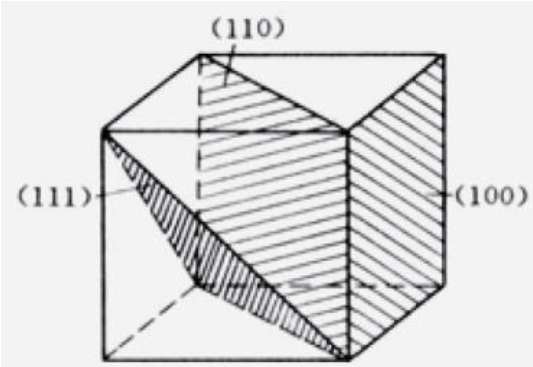
\includegraphics[width=7cm]{Fig/2.5.png}
        \caption{晶面指数}
    \end{figure}
    \par \hspace*{2em}组成晶体的原子可以看成分别作处在一系列相
    互平行而且间距一定的平面族上,这些平面称为晶面。晶面有许多不同的取法。
    \par \hspace*{2em}三维空间中原子组成的格点,可看作是一个三维的光栅网络。晶体对电子波衍射
    的实质是每个格点上的原子产生的散射波的相干叠加。它们的相干叠加的第一步可看作是同一
    晶面上各个原子发出的散射波的相干叠加,形成每一个晶面的衍射波;第二步是同一晶面族的
    不同晶面的衍射波之间的相干叠加。满足
    \begin{equation}
        2d\sin \theta =k\lambda,k=1,2,3...
    \end{equation}
    时,才能形成干涉极大。此方程称为晶体衍射的布拉格条件。如果改成通常习惯使用的入射
    角$\beta$表示,布拉格条件可写为:
    \begin{equation}{\label{eqn-2}}
        2d\cos \beta =k\lambda,k=1,2,3...
    \end{equation}
    \par \hspace*{2em}如果布拉格条件得到满足,每一
    个晶面族在特定方向产生一个衍射极大,从实验上测得衍射极大的方向角$\beta$,并且知道波长$\lambda$,
    从布拉格条件可求出晶面间距$d$ ,通过进一步分析可以确定晶格常数$a$ 。反之,若已知晶格常
    数$a$ ,可求出波长$\lambda$。
    \par \hspace*{2em}实际晶体的晶格常数为$10^{-10}m$ 数量级,为了观察到晶体对电磁波的衍射,晶格常数与电磁
    波的波长必须是同一数量级,也就是说使用X射线进行衍射。实际上X射线衍射仪较贵,本实验采用分米级的晶体模型模拟实验。
    晶体模型中,使用铝制小球模拟原子。
    \item 微波的双缝干涉实验
    \par \hspace*{2em} 当一平面波垂直入射到一金属板的两条狭缝上,狭缝就成为次级波波源。由两缝发出的次
    级波是相干波,因此在金属板的背后面空间中,将产生干涉现象。当然,波通过每个缝都有衍射
    现象。因此实验将是衍射和干涉两者结合的结果。为了只研究主要来自两缝中央衍射波相互干
    涉的结果,要让双缝间距b较小,单缝的宽度a接近波长。
    \newline 干涉加强的角度为
    \begin{equation}{\label{eqn-3}}
        \varphi =\sin^{-1}\left(\frac{k\cdot \lambda}{a+b}\right),k=1,2,3...
    \end{equation}
    \newline 干涉减弱的角度为
    \begin{equation}{\label{eqn-4}}
        \varphi =\sin^{-1}\left(\frac{2k+1}{2}\cdot \frac{\lambda}{a+b}\right),k=1,2,3...
    \end{equation}
    \item 微波的单缝衍射实验
    \par \hspace*{2em} 当一平面微波入射到一宽度和微波波长可比拟的一狭缝时,在缝后就要发生如光波一般的衍
    射现象。同样中央零级最强,也最宽,在中央的两侧衍射波强度将迅速减小。
    \begin{figure}[H]
        \centering
        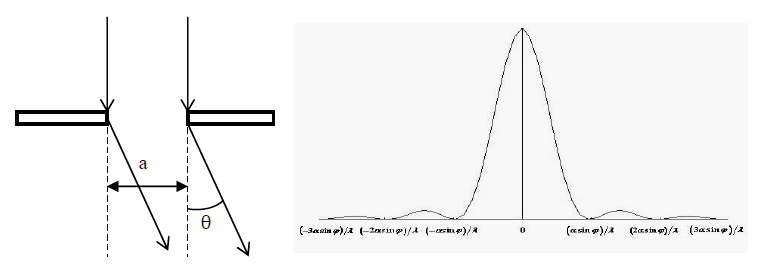
\includegraphics[width=10cm]{Fig/3.png}
        \caption{干涉和干涉强度示意图}
    \end{figure}
    \hspace*{2em}根据光的单缝衍射公式推导可知,如为一维衍射,微波单缝衍射图样的强度分布规律也为:
    \begin{equation}{\label{eqn-5}}
        I=I_0\frac{\sin^2\mu}{\mu^2} \qquad \mu=\frac{\pi a \sin\varphi }{\lambda}
    \end{equation}
    \hspace*{2em}式中$I_0$ 是中央主极大中心的微波强度,$a$为单缝的宽度,$\lambda$是微波的波长,$\varphi$为衍射角,
    $\frac{\sin^2\mu}{\mu^2}$常叫做单缝衍射因子,表征衍射场内任一点微波相对强度的大小。一般可通过测量衍射屏上从中央向两边微波强度变化来验证公式\eqref{eqn-5}。同时与光的单缝衍射一样,当
    \begin{equation}{\label{eqn-6}}
        a\sin\varphi=\pm k\lambda,k=1,2,3...
    \end{equation}
    时,相应的$\varphi$角位置衍射度强度为零。如测出衍射强度分布,则可依据第一级衍射最
    小值所对应的$\varphi$角度,利用公式\eqref{eqn-6},求出微波波长$\lambda$ 。
    \item 微波的迈克尔逊干涉实验
    \begin{figure}[H]
        \centering
        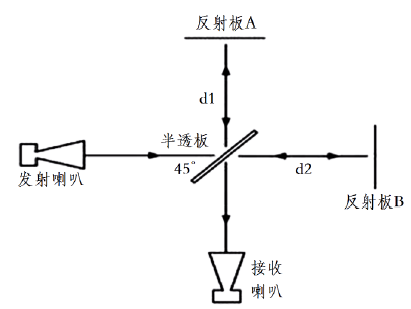
\includegraphics[width=6.5cm]{Fig/4.png}
        \caption{迈克尔逊干涉示意图}
        \label{迈克尔逊干涉}
    \end{figure}
    \hspace*{2em} 在微波前进的方向上放置一个与波传播方向成$45^\circ$角的半透射半反射的分束板(如\cref{迈克尔逊干涉})。将
    入射波分成一束向金属板A 传播,另一束向金属板B 传播。由于A、B 金属板的全反射作用,
    两列波再回到半透射半反射的分束板,回合后到达微波接收器处。这两束微波同频率,在接收
    器处将发生干涉,干涉叠加的强度由两束波的程差(即位相差)决定。当两波的相位差为
    $2k\pi,k=\pm1,\pm2,\pm3...$
    时,干涉加强;当两波的相位差为$\left(2k+1\right)\pi,k=\pm1,\pm2,\pm3...$时,则干涉最弱。当 A、
B 板中的一块板固定,另一块板可沿着微波传播方向前后移动,当微波接收信号从极小(或极
大)值到又一次极小(或极大)值,则反射板移动了$\frac{\lambda}{2}$距离。由这个距离就可求得微波波长。

\end{enumerate}

\section{实验内容}

\subsection{实验条件确认}
\begin{enumerate}
    
    
    \item 实验条件:\hspace{2em} 微波频率:$f_0=9.4GHz$ \hspace{2em} 微波波长:$\lambda_0=3.2cm$
    \item 微波实验仪对准试验
    \par \hspace*{2em}调整仪器喇叭使其处于水平/竖直状态。调整刻度盘使$180^\circ$刻度指向微波发射喇叭。调整输出电压使接收到的最大电压在150mV左右,移动接收喇叭到$\pm 20^\circ$位置,使两位置电压偏差在2\%以内。
    \begin{table}[H]
        \centering
        \caption{微波实验仪对准确认}
        \begin{tabularx}{0.5\textwidth}{|X|X|X|X|}\hline
            角度$(^\circ)$  &  0  &  20  &  -20  \\\hline
            电压(mV)  &  149  &  106  &  104  \\\hline
            
        \end{tabularx}
        
    \end{table}
    
\end{enumerate}
\subsection{双缝干涉实验}
\noindent 实验步骤:
\begin{enumerate}
    \item 调整双缝板缝宽$a=3.5cm$,缝间距$b=5cm$。
    \item 将双缝干涉板安置在支座上,使双缝板平面与载物圆台上$90^\circ$指示线一致。再次调整摇臂角度至$\pm20^\circ$,确保两侧读数大致一致。
    \item 以$2^\circ$为间隔,测量$-50^\circ\thicksim 50^\circ$的光强分布,并记录。(注:光强以接收端电压的形式记录,能够良好表达光强比例,但不能表示实际光强。)
    \item 根据测量数据,寻找一级极大、零级极小、一级极小,以$1^\circ$为间隔在出现上述极值的区域内测量,寻求极值所在的度数。(此处未增大功率)
\end{enumerate}
\noindent 实验数据:
        % Table generated by Excel2LaTeX from sheet 'Sheet1'
        \begin{table}[H]
          \centering
          \caption{微波双缝干涉实验数据}
            \begin{tabularx}{0.75\textwidth}{|c|X|X|X|X|X|X|X|X|X|}\hline
            $\theta(^\circ)$      & 0      & 2      & 4      & 6      & 8      & 10     & 12     & 14     & 16 \\\hline
            $U_{\theta+}(mV)$     & 149    & 137    & 100    & 23.7   & 0.2    & 0.6    & 9.5    & 46     & 88 \\\hline
            $U_{\theta-}(mV)$    & 149    & 160    & 161    & 122    & 34     & 3.4    & 2.2    & 31     & 69 \\\hline
            $\theta(^\circ)$      & 18     & 20     & 22     & 24     & 26     & 28     & 30     & 32     & 34 \\\hline
            $U_{\theta+}(mV)$      & 100    & 105    & 86     & 49     & 14     & 2.9    & 2.1    & 2.6    & 7.7 \\\hline
            $U_{\theta-}(mV)$     & 79     & 101    & 124    & 117    & 81     & 30     & 7.1    & 4.4    & 6.9 \\\hline
            $\theta(^\circ)$      & 36     & 38     & 40     & 42     & 44     & 46     & 48     & 50     & 52 \\\hline
            $U_{\theta+}(mV)$      & 76     & 15     & 6      & 11.7   & 15     & 32     & 23     & 3.9    & 0.9 \\\hline
            $U_{\theta-}(mV)$     & 16.6   & 30     & 26     & 6.8    & 2.2    & 22.5   & 50     & 37.6   & 8.6 \\\hline
            \end{tabularx}%
          \label{tab:双缝干涉}%
        \end{table}%
        \begin{figure}[H]
            \centering
            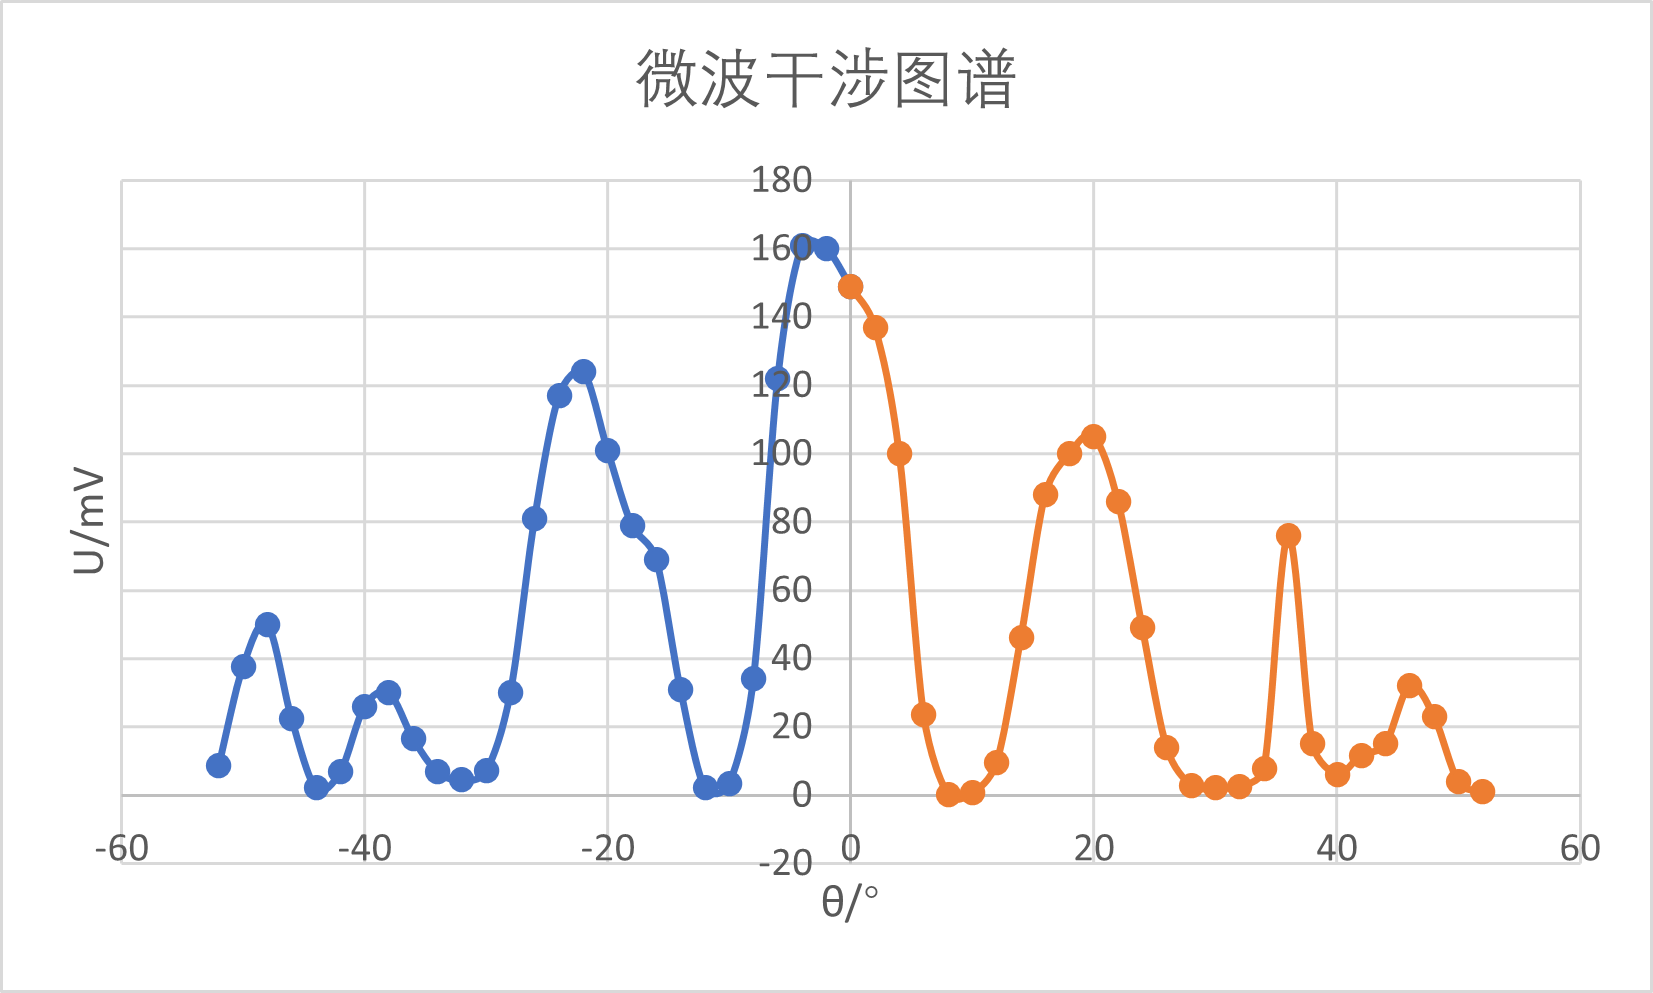
\includegraphics[width=7cm]{Fig/5.png}
            \caption{双缝干涉图谱}
        \end{figure}
    可以看到,图像左半边也就是$\theta<0$的光强测量误差较大,左侧二级极大小于三级极大,同时0极极大出现在左半边而不是$0^\circ$。可能的原因在误差分析中讨论。
    \begin{table}[H]
        \centering
        \caption{一级极大}
        \begin{tabular}{|c|c|c|c|c|c|c|c|c|c|}
        \hline
            $U_{\theta +}/mV$ & 93 & 98 & 101 & 98 & 82 & 72 & 52 & 31 & 18 \\ \hline
            $\theta /^\circ$ & 18 & 19 & 20 & 21 & 22 & 23 & 24 & 25 & 26 \\ \hline
            $U_{\theta -}/mV$ & 74.4 & 82 & 95 & 108 & 123 & 125 & 115 & 103 & 75 \\ \hline
        \end{tabular}
    \end{table}
    \begin{table}[H]
        \centering
        \caption{零级极小}
        \begin{tabular}{|c|c|c|c|c|c|c|c|c|c|}
        \hline
            $\theta /^\circ$ & 6 & 7 & 8 & 9 & 10 & 11 & 12 & 13 & 14 \\ \hline
            $U_{\theta +}/mV$ & 27 & 4.5 & 0.7 & 0.1 & 0.6 & 1.4 & 9.1 & 15 & 32 \\ \hline
            $\theta /^\circ$ & -6 & -7 & -8 & -9 & -10 & -11 & -12 & -13 & -14 \\ \hline
            $U_{\theta -}/mV$ & 111 & 86 & 41 & 13 & 2.9 & 1.2 & 1.9 & 5.6 & 24.9 \\ \hline
        \end{tabular}
    \end{table}
    \begin{table}[!ht]
        \centering
        \caption{一级极小}
        \begin{tabular}{|c|c|c|c|c|c|c|c|c|c|}
        \hline
            $\theta /^\circ$ & 27 & 28 & 29 & 30 & 31 & 32 & 33 & 34 & 35 \\ \hline
            $U_{\theta +}/mV$ & 10 & 4 & 2.3 & 1.9 & 1.6 & 2.2 & 4 & 9 & 12 \\ \hline
            $\theta /^\circ$ & -29 & -30 & -31 & -32 & -33 & -34 & -35 & -36 & -37 \\ \hline
            $U_{\theta -}/mV$ & 11.2 & 5.7 & 4.2 & 4 & 4.8 & 6.6 & 9.1 & 14.2 & 22.7 \\ \hline
        \end{tabular}
    \end{table}
    由此可见,一级极大为$+20^\circ, -23^\circ\approx 21.5^\circ$,零级极小为$+9^\circ, -11^\circ\approx 10^\circ$,一级极小为$+31^\circ, -32^\circ\approx 31.5^\circ$。
    由公式\eqref{eqn-3}\eqref{eqn-4}
    \begin{equation}
        \lambda=\frac{1}{k}\sin\varphi \cdot\left(a+b\right)\text{(光强极大时)}=\frac{2}{2k+1}\sin\varphi \cdot \left(a+b\right)\text{(光强极小时)}
    \end{equation}
    \hspace*{2em}于是$\lambda_1=3.12cm,\lambda_2=2.95cm,\lambda_3=2.96cm$,平均值为$\lambda=3.01cm$。与理论值$\lambda_0=3.2cm$的误差为$6\%$。
    \newline \hspace*{2em}将此部分数据替换原表\ref{tab:双缝干涉}中对应的数据,生成新的曲线。
    \begin{figure}[H]
        \centering
        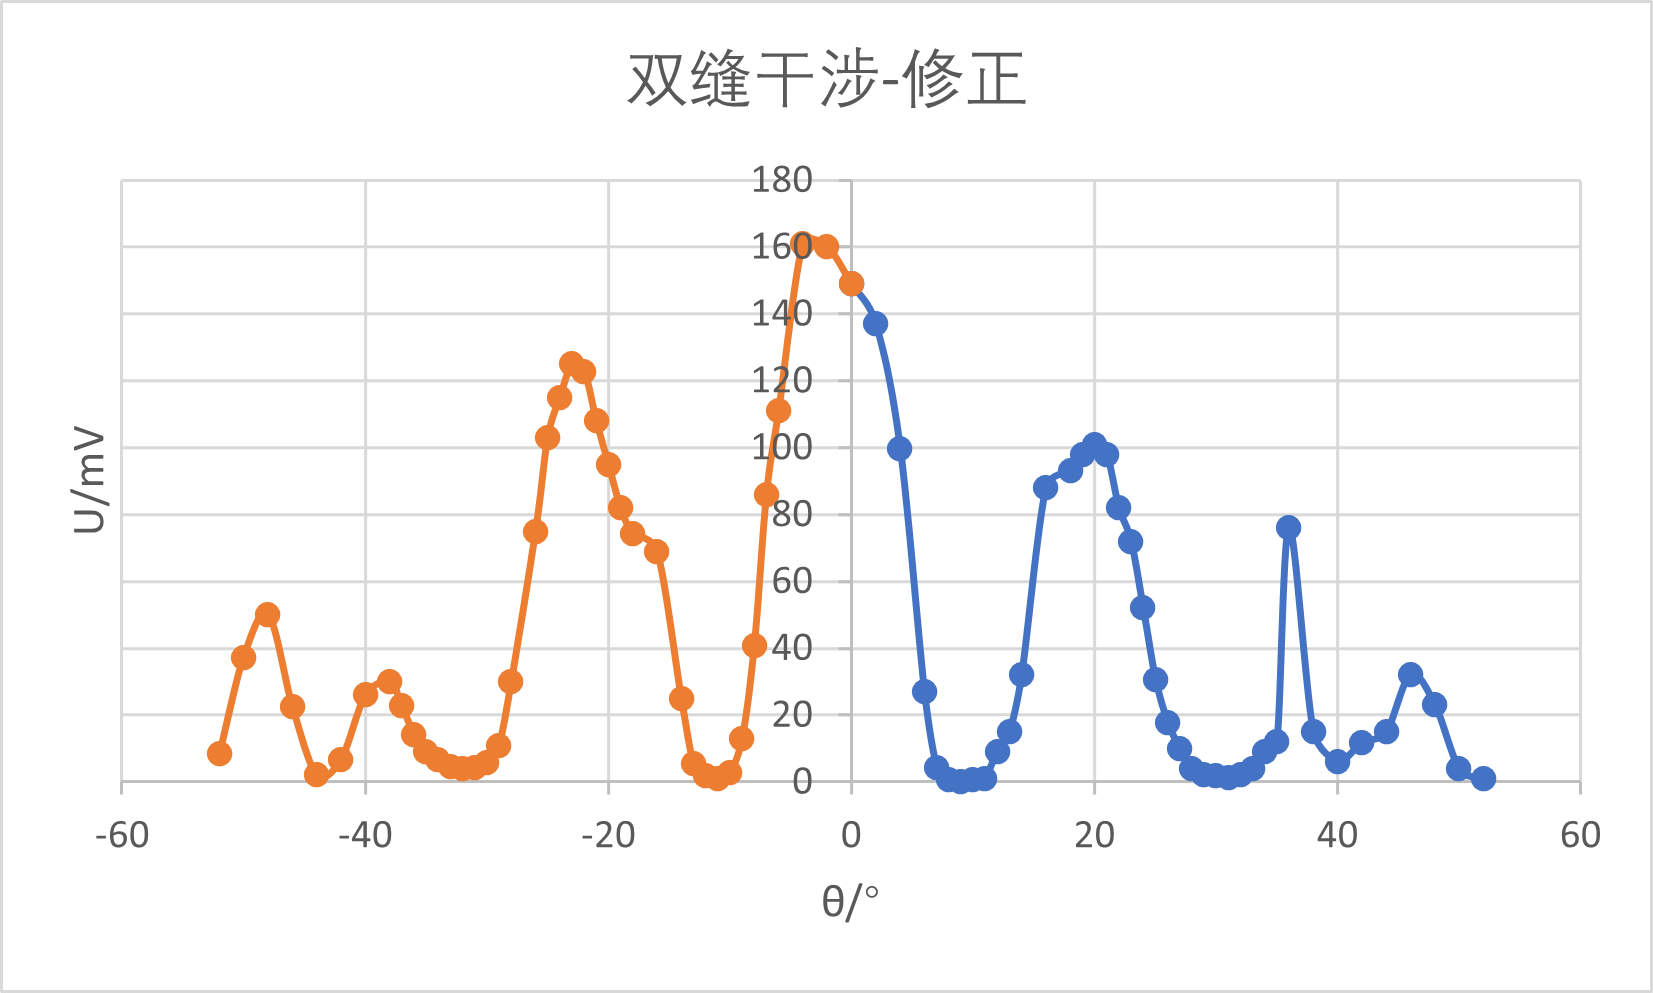
\includegraphics[width=7cm]{Fig/6.png}
        \caption{双缝干涉图谱-修正}
    \end{figure}
    左侧二级极大点仍旧缺失,修正后的图像效果未变好。
\subsection{微波单缝衍射实验}
\noindent 实验步骤:
\begin{enumerate}
    \item 微波实验仪对准确认(加单缝前)(如5.1.2)。
    \begin{table}[H]
        \centering
        \caption{微波实验仪对准确认(加单缝前)}
        \begin{tabularx}{0.5\textwidth}{|X|X|X|X|}\hline
            角度$(^\circ)$  &  0  &  20  &  -20  \\\hline
            电压(mV)  &  173  &  10  &  10  \\\hline
        \end{tabularx}  
    \end{table}
    \item 调整单缝板缝宽$a=8cm$。
    \item 将单缝衍射板安置在支座上,使单缝板平面与载物圆台上$90^\circ$指示线一致。再次调整摇臂角度至$\pm10^\circ$,确保两侧读数大致一致。($\pm20^\circ$时度数小)
    \item 以$2^\circ$为间隔,测量$-40^\circ\thicksim 40^\circ$的光强分布,并记录。(注:光强以接收端电压的形式记录,能够良好表达光强比例,但不能表示实际光强。)
    \item 根据测量数据,寻找极小值,增大功率,以$1^\circ$为间隔在出现上述极值的区域内测量,寻求极值所在的度数。
\end{enumerate}
\noindent 实验数据:
\begin{table}[!ht]
    \centering
    \caption{微波单缝衍射实验数据}
    \begin{tabular}{|c|c|c|c|c|c|c|c|c|c|c|c|}
    \hline
        $\theta /^\circ$ & 0 & 2 & 4 & 6 & 8 & 10 & 12 & 14 & 16 & 18 & 20 \\ \hline
        $U_{\theta +}/mV$ & 142 & 148 & 155 & 142 & 101 & 51 & 23 & 11.9 & 5.5 & 1.3 & 0.1 \\ \hline
        $U_{\theta -}/mV$ & 141 & 143 & 153 & 160 & 137 & 99 & 52 & 25 & 14 & 6 & 1.1 \\ \hline
        $\theta /^\circ$ & 22 & 24 & 26 & 28 & 30 & 32 & 34 & 36 & 38 & 40 & ~ \\ \hline
        $U_{\theta +}/mV$ & 0.1 & 0.1 & 0.1 & 0.3 & 1.3 & 2.3 & 1.4 & 0.2 & 0.2 & 0.4 & ~ \\ \hline
        $U_{\theta -}/mV$ & 0 & 0 & 0.1 & 0.1 & 0.1 & 0.6 & 1.5 & 1.2 & 0.3 & 0.1 & ~\\ \hline
    \end{tabular}
\end{table}
\begin{figure}[H]
    \centering
    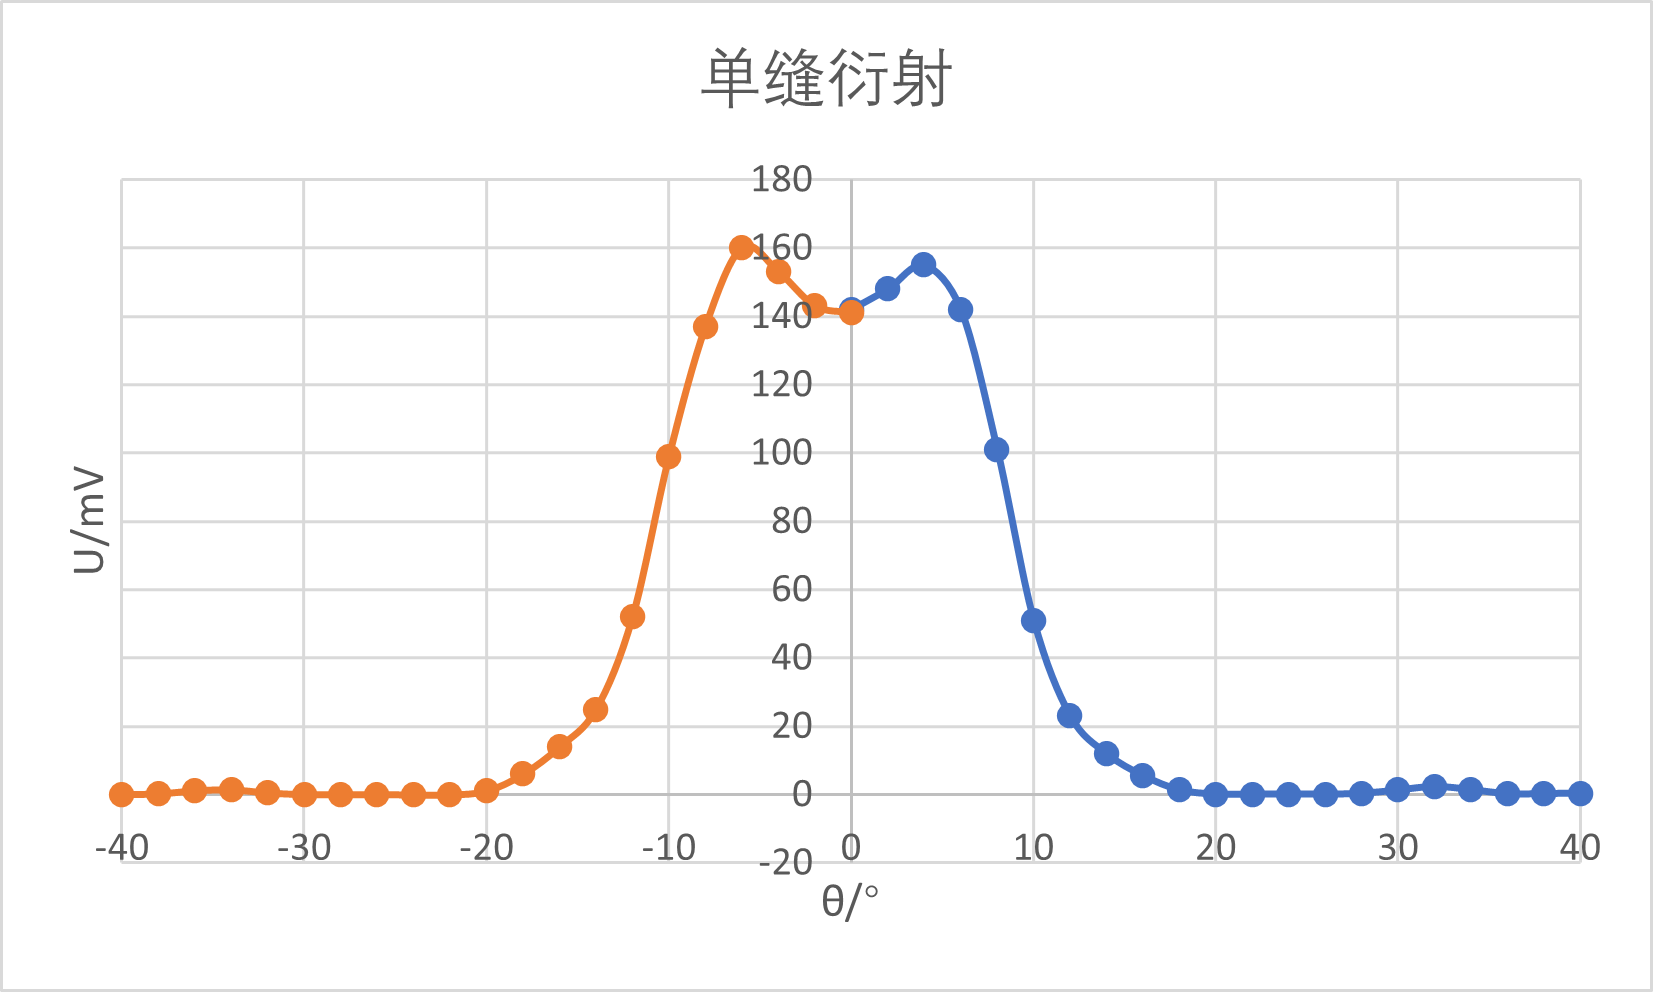
\includegraphics[width=7cm]{Fig/7.png}
    \caption{单缝衍射图谱}
\end{figure}
\begin{table}[!ht]
    \centering
    \caption{一级极小}
    \begin{tabular}{|c|c|c|c|c|c|c|c|c|c|}
    \hline
        $\theta /^\circ$ & 19 & 20 & 21 & 22 & 23 & 24 & 25 & 26 & 27 \\ \hline
        $U_{\theta +}/mV$ & 2.9 & 0.6 & 0.1 & 0.2 & 0.6 & 0.6 & 0.9 & 0.5 & 0.5 \\ \hline
        $U_{\theta -}/mV$ & 39.1 & 22 & 3.3 & 0.4 & 0.1 & 0 & 0.2 & 0.4 & 0.5 \\ \hline
    \end{tabular}
\end{table}
    可见,一级极小为$+21^\circ, -24^\circ\approx 22.5^\circ$。
    \newline \hspace*{2em}由公式\eqref{eqn-3}
    \begin{equation}
        \lambda=\frac{1}{k}\sin\varphi \cdot a
    \end{equation}
    \hspace*{2em}于是$\lambda_4=3.06cm$,与理论值$\lambda_0=3.2cm$的误差为$4.4\%$。

\subsection{微波迈克尔逊干涉实验}
\noindent 实验步骤:
\begin{enumerate}
    \item 微波实验仪姿态确认(如5.1.2)(具体数据略)。
    \item 将玻璃板安装在支座上,使玻璃板面与载物圆台$45^\circ$线在统一面上。固定臂指针指向$180^\circ$刻度线,接收臂指针指向$90^\circ$刻度线。(如图\ref{迈克尔逊干涉})
    \item 安装两个反射板,分别在指针指向$0^\circ$和$90^\circ$。扭动千分尺旋钮至0刻度。
    \item 扭动千分尺旋钮,在接收端示数极小时进行度数,进行四次测量。
\end{enumerate}
\noindent 实验数据:
\begin{table}[H]
    \centering
    \caption{迈克尔逊干涉最小点度数}
    \begin{tabularx}{0.6\textwidth}{|c|X|X|X|X|}
    \hline
        最小点度数/cm & 1.187 & 2.840 & 4.434 & 6.097  \\ \hline
    \end{tabularx}
\end{table}
    由逐差法计算,
    \begin{equation}
        \Delta=\frac{(x_3+x_4)-(x_1+x_2)}{4}=1.626cm=\frac{\lambda}{2}
    \end{equation}
    计算得$\lambda=3.25cm$,与理论值$\lambda_0=3.2cm$的误差为$1.6\%$。

\subsection{微波布拉格衍射}
\noindent 实验步骤:
\begin{enumerate}
    \item 微波实验仪姿态确认(如5.1.2)(具体数据略)。
    \item 将晶体模型安装在支座上。根据所测晶面选择法线角度(100——$\mathbf{90^\circ}$,110——$\mathbf{45^\circ}$)。
    \item 根据所测角度调整固定臂和接收臂与法线的角度,依照表格进行测量。
    \item 根据测量数据,寻找极小值,增大功率,以$1^\circ$为间隔在出现上述极值的区域内测量,寻求极值所在的度数。
\end{enumerate}
\noindent 实验数据:
\par
1.100晶面\qquad 面间距$d=4cm$\qquad $\varphi$为入射角度(反射角度)
\begin{table}[H]
    \centering
    \caption{布拉格衍射数据(100)晶面}
    \begin{tabular}{|c|c|c|c|c|c|c|c|c|c|}
    \hline
        $\varphi /^\circ$ & 30 & 32 & 34 & 36 & 38 & 40 & 42 & 44 & 46 \\ \hline
        $U/mV$ & 8.7 & 3.8 & 7 & 9 & 16.1 & 26.1 & 13.9 & 3 & 5.4 \\ \hline
        $\varphi /^\circ$ & 48 & 50 & 52 & 54 & 56 & 58 & 60 & 62 & 64 \\ \hline
        $U/mV$ & 27.9 & 25.6 & 0.5 & 1.1 & 4.2 & 0.7 & 32 & 18.9 & 9.1 \\ \hline
        $\varphi /^\circ$ & 66 & 68 & 70 & 72 & 74 & 76 & 78 & 80 & ~ \\ \hline
        $U/mV$ & 114 & 158 & 1.9 & 4.1 & 14.8 & 27.4 & 7.2 & 37.4 & ~\\ \hline
    \end{tabular}
\end{table}
\begin{table}[H]
    \centering
    \caption{(100)晶面极大值}
    \begin{tabular}{|c|c|c|c|c|c|c|c|c|c|}
    \hline
        $\varphi /^\circ$ & 65 & 66 & 67 & 68 & 69 & 70 & 71 & 72 & 73 \\ \hline
        $U/mV$ & 74.8 & 125 & 169 & 145 & 58 & 0.6 & 1.5 & 3.6 & 1 \\ \hline
    \end{tabular}
\end{table}
\par 极大值时,$\varphi=67^\circ$。在已知晶面间距$d$的情况下,由公式\eqref{eqn-2},
\begin{equation}{\label{eqn-10}}
    \lambda=2d\cos\varphi
\end{equation}
\par 于是$\lambda_5=3.13cm$,与理论值$\lambda_0=3.2cm$的误差为$2.2\%$。、
\par 在已知波长$\lambda$的情况下,由公式\eqref{eqn-2}
\begin{equation}{\label{eqn-11}}
    d=\frac{\lambda}{2\cos \varphi} 
\end{equation}
\par 于是$d=4.09cm$,与理论值$d_0=4cm$的误差为$2.3\%$。

\par
2. 110晶面\qquad 面间距$d=2.828cm$\qquad $\varphi$为入射角度(反射角度)
\begin{table}[H]
    \centering
    \caption{布拉格衍射数据(110)晶面}
    \begin{tabular}{|c|c|c|c|c|c|c|c|c|c|c|c|}
    \hline
        $\varphi /^\circ$ & 30 & 32 & 34 & 36 & 38 & 40 & 42 & 44 & 46 & 48 & 50 \\ \hline
        $U/mV$ & 0.2 & 0.6 & 1.1 & 0.7 & 0.3 & 1.8 & 1.7 & 8.9 & 12.2 & 6.5 & 28.1 \\ \hline
        $\varphi /^\circ$ & 52 & 54 & 56 & 58 & 60 & 62 & 64 & 66 & 68 & 70 & ~ \\ \hline
        $U/mV$ & 70.1 & 119 & 92 & 71 & 43 & 0 & 4.5 & 1.5 & 0.2 & 0.3 & ~ \\ \hline
    \end{tabular}
\end{table}
\begin{table}[H]
    \centering
    \caption{(110)晶面极大值}
    \begin{tabular}{|c|c|c|c|c|c|c|c|c|c|}
    \hline
        $\varphi /^\circ$ & 50 & 51 & 52 & 53 & 54 & 55 & 56 & 57 & 58 \\ \hline
        $U/mV$ & 27 & 55 & 75 & 109 & 141 & 127 & 101 & 85 & 82 \\ \hline
    \end{tabular}
\end{table}
    \par 极大值时,$\varphi=54^\circ$。
    \par 在已知晶面间距$d$的情况下,由公式\eqref{eqn-10},于是$\lambda_5=3.13cm$,与理论值$\lambda_0=3.2cm$的误差为$2.2\%$。
    \par 在已知波长$\lambda$的情况下,由公式\eqref{eqn-11},于是$d=2.722cm$,与理论值$d_0=2.828cm$的误差为$3.7\%$。

\begin{figure}[H]
    \begin{minipage}[t]{0.49\linewidth}
        \centering
        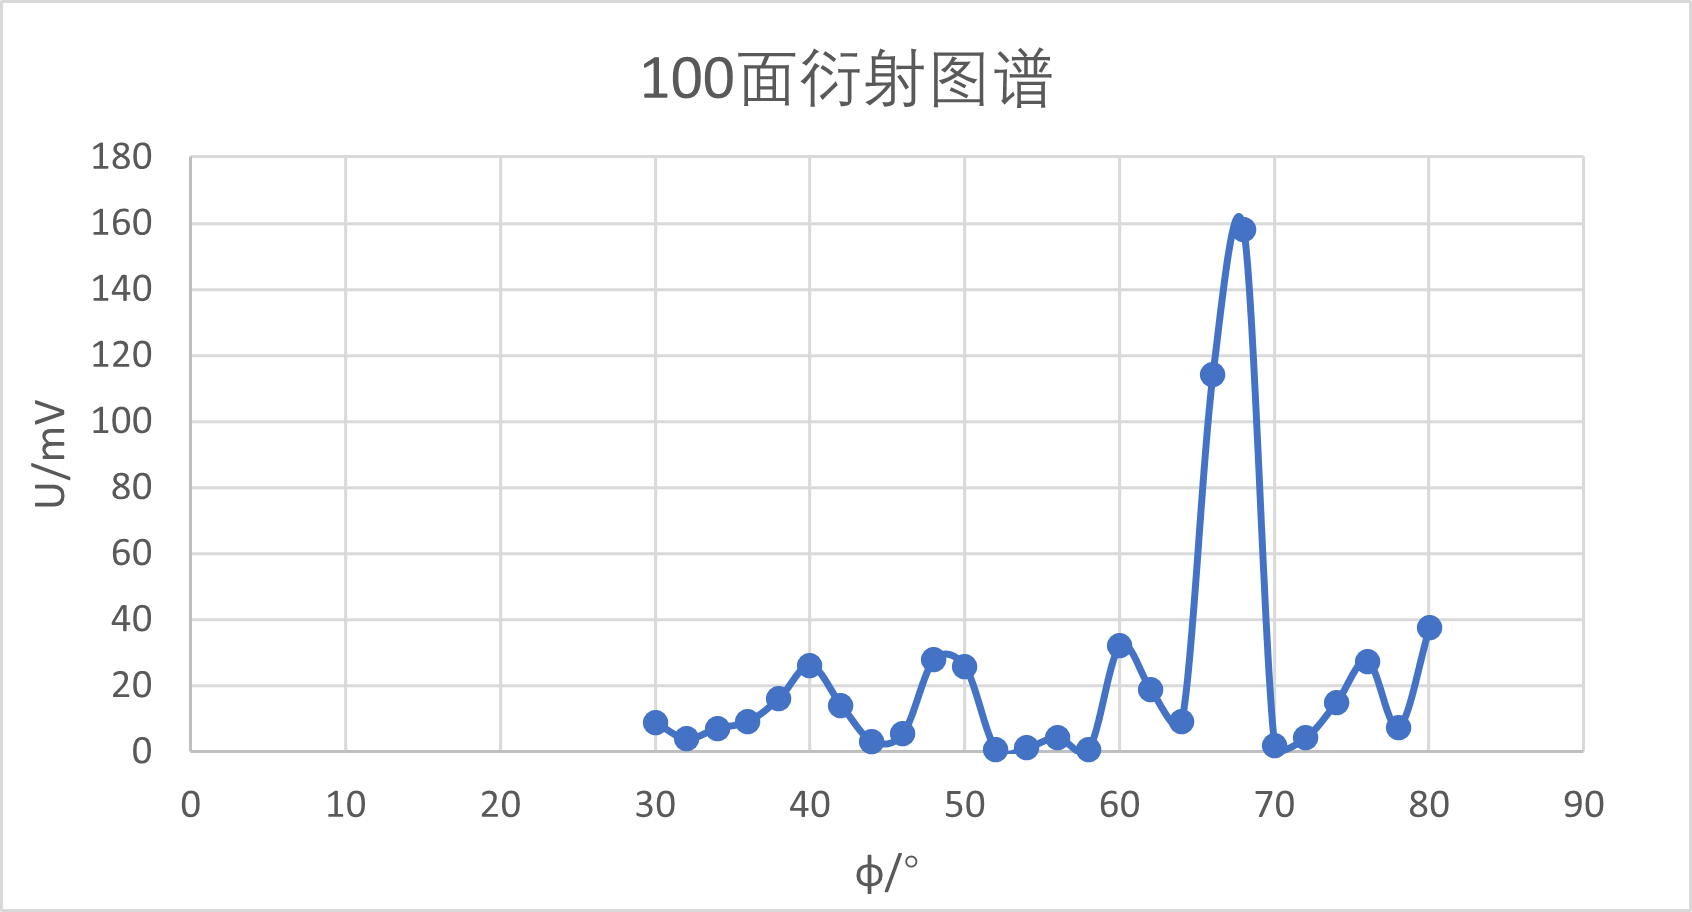
\includegraphics[width=7.5cm]{Fig/8.png}
        \caption{(100)面衍射图谱}
    \end{minipage}
    \begin{minipage}[t]{0.49\linewidth}
        \centering
        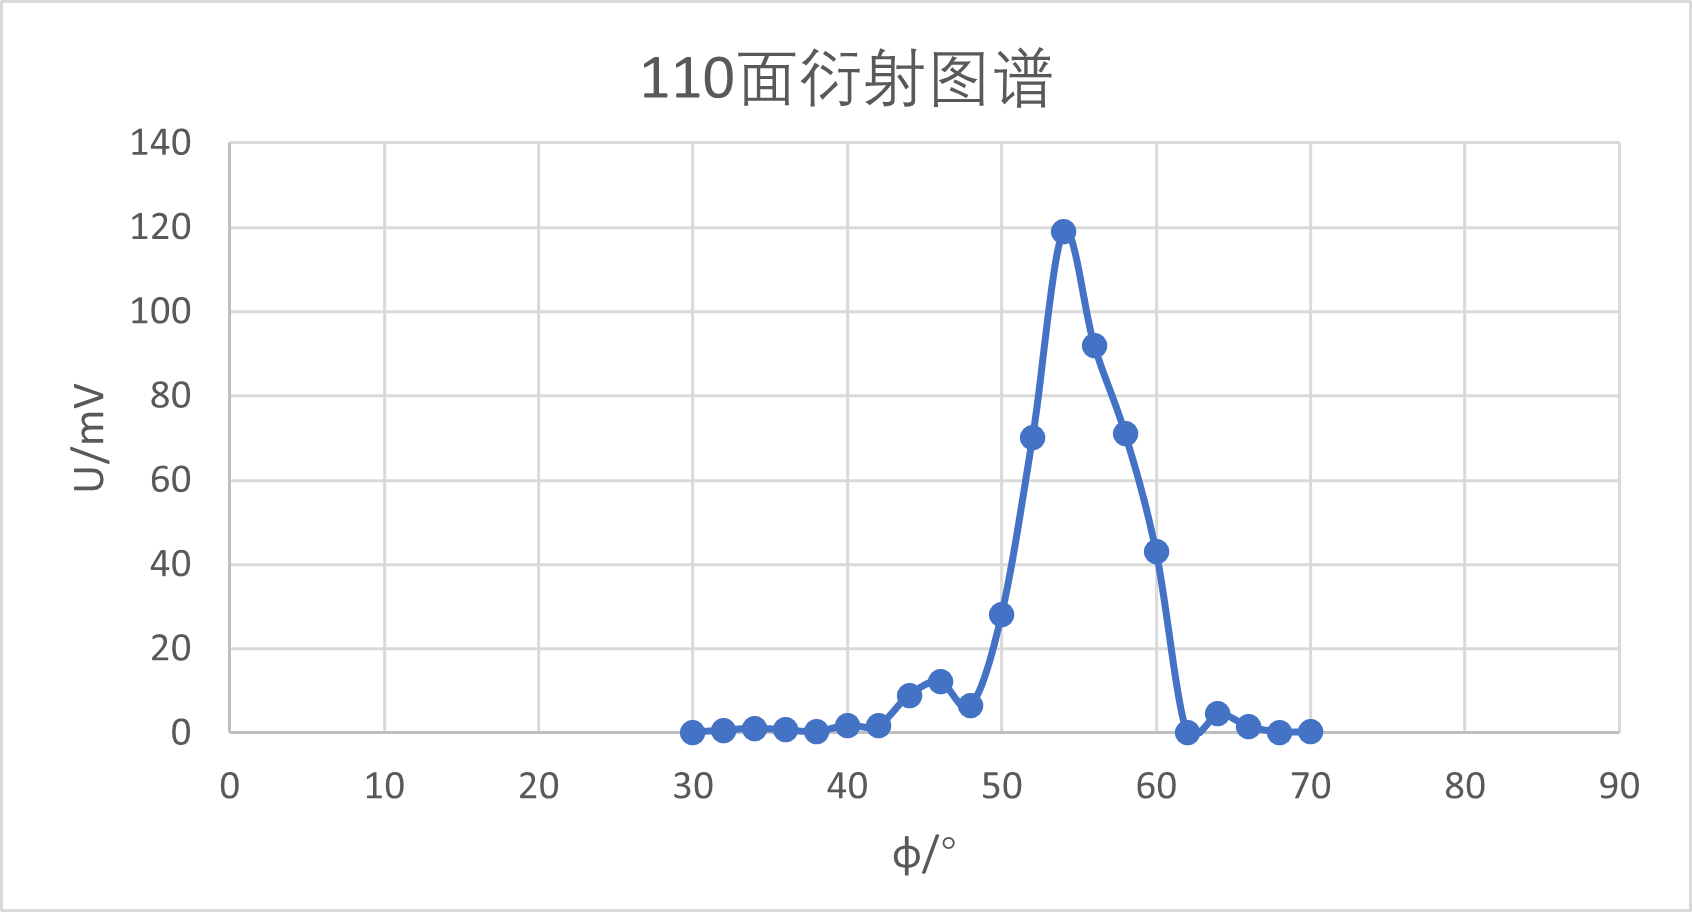
\includegraphics[width=7.5cm]{Fig/9.png}
        \caption{(110)面衍射图谱}
    \end{minipage}
\end{figure}


\section{实验反思、收获与总结}
\noindent 思考题:
\begin{enumerate}
    \item 各实验内容误差主要影响是什么?
    \par  (1)输出喇叭输出的波长本身具有误差。
    \par  (2)输出端和接收端喇叭未恰好垂直,造成误差。
    \par  (3)实验仪器安装时,微小的角度偏差造成的测量误差。
    \par  (4)实验操作台过小,导致很容易在转大角度时摇臂碰到插线板/边缘,导致摇臂上的喇叭发生角度变化,造成一套测量中的后续误差。此误差为操作上的误差,在单缝衍射/双缝干涉这样的多组测量实验中较为明显。
    \par  (5)实验台摇臂长度有限,并且角度盘的分度值为$1^\circ$,因此调整仪器时角度上的微小误差无法避免,读取角度可能比实际角度偏大/偏小。
    \par  (6)双缝干涉实验中,半波长度较小,测量时很难恰好取到极值,很可能取到的极值为真实极值的0.5—1倍。因此实验数据中会出现三级极大比二级极大大的情况。
    \par  (7)微波迈克尔逊干涉中,千分尺具有问题。旋转方向与刻度增大的方向相反,因此需要对千分尺读数取余数。由于千分尺长度有限,只能测量4-5组数据,若测量数据在6组以上,在逐差法下测量误差会显著降低。
    \par  (8)微波布拉格衍射中误差较小,因为测量分度值为$2^\circ$,同时调整入射角和反射角后等价于每次调整$4^\circ$,操作误差造成的影响小。
    \item 金属是一种良好的微波反射器。其它物质的反射特性如何?是否有部分能量透过这些物质还是被吸收了?比较导体与非导体的反射特性。
    \par \hspace*{2em} 微波反射率与物体的材料属性、表面形态、入射角度和频率等因素密切相关。首先,不同材料对微波的反射率有所差异。金属通常具有较高的反射率,这是因为金属的电导率较高,微波在金属表面遇到导电体时会被反射。而绝缘体的反射率较低,微波在绝缘体表面遇到非导电体时,会被一部分吸收,一部分反射。其次,物体表面形态对微波反射率也有影响。表面粗糙的物体会使微波的反射率增加,因为粗糙表面会使微波在入射时发生多次反射,增加了反射的机会。而平滑表面的物体,微波反射率较低,因为微波在入射时很少发生反射。此外,入射角度也会影响微波反射率。一般来说,入射角度越小,反射率越低,因为入射角度较小时,微波更容易进入物体内部,减少了反射。最后,微波的频率也会影响反射率。不同频率的微波在物体表面的反射能力有所差异,不同频率下的反射率也不相同。
    \par \hspace*{2em} 对于玻璃、塑料和瓷器,微波几乎是穿越而不被吸收。对于水和食物等就会吸收微波而使自身发热。而对金属类东西,则会完全反射微波。微波能穿透生物体表层,穿透深度与波长是同量级的,医学界常用微波做表层加热治疗。在可发射可接受的无线电波中,只有微波能穿透电离层,于是人类用微波探测外层空间,射电望远镜就是用来发射和接受外太空的微波的。毫米波还能穿透等离子体,是远程导弹和航天器重返大气层时实现通信和末端制导的重要手段。
    \par \hspace*{2em} 不同物质对微波的吸收程度不同,产生的热效果也不同,于是微波加热就表现出选择性加热的特点了。水分子属电极性分子,对微波具有强吸收能力。而蛋白质、碳水化合物对微波的吸收能力比水小得多。因此,对于食品来说,含水量的多少对微波加热效果影响很大,含水量大的微波加热效果好。
    \item 为避免每台仪器微波间的干扰,使用吸波材料对每套设备进行了微波屏蔽,请问吸波材料的工作机理是什么?与屏蔽微波波长的关系是什么?
    \par \hspace*{2em} 部分内容见4.1。
    \par \hspace*{2em} 吸收微波的基本原理是通过某种物理作用机制将微波能转化为其他形式运动的能量,并通过该运动的耗散作用而转化为热能。微波激发的一切形式的有耗运动皆可成为吸收机制。常见的机制有电感应、磁感应、电磁感应,以及电磁散射等。实际应用的微波吸收材料常常可能有多种机制起作用。
    \par \hspace*{2em} 微波吸收材料应具有良好的吸波性能,即有高于要求的阈值的微波吸收率和宽的吸收频带。本实验采用了吸收型微波吸收材料(泡沫吸收材料)。这类吸收泡沫多用于各种微波暗室,基体材料多用聚氨酯(PU)多做成椎体形状,用来吸收不同角度的电磁波,重量轻、柔性好,比较容易剪裁。椎体长度要求$\frac{L}{\lambda}\approx 1$。
    \item 假如预先不知道晶体中晶面的方向,是否会增加实验的复杂性?又该如何定位这些晶面?
    \par \hspace*{2em} 会增加实验的复杂性。首先需要确认晶体的一个晶面法线方向。考虑$0^\circ$入射,$180^\circ$接收,旋转晶体模型,当接收端处于极小值时为晶面法线方向。然后,将晶体模型旋转$90^\circ$,此时接收端处于极大值,为晶面法线方向。最后,将晶体模型旋转$45^\circ$,此时接收端处于极小值,为晶面法线方向。由此可知,晶体中晶面的方向可以通过旋转晶体模型,观察接收端的极大值和极小值来确定。
    \par \hspace*{2em} 对不同晶面族,根据上述方法取到的晶面方向进行测量,固定入射波长,比较所得的d的比值,由$\sqrt{n_x^2+n_y^2+n_z^2}$的比值,能够确定所测的晶体族。

\end{enumerate}
\noindent 个人反思:
\begin{enumerate}
    \item 在第一次测量双缝干涉数据时,我进行了重测,由于实验数据极为不对称。在安装干涉/衍射板时一定要尽量垂直,并且确认好两个喇叭的初始位置良好,尽量与摇臂垂直。尽管如此,还是会造成实验数据不对称,在$\pm 2^\circ$内即可接受。
    \item 在迈克尔逊干涉实验中,根据高中力学测量加速度的经验,直接想到了逐差法进行数据处理,这很好的降低了误差。
    \item 在双缝干涉实验中,衍射效应也很明显。考虑二级极大,一级极小和二级极小的间距差
    \[\Delta \theta =\arcsin\left(2k\frac{\lambda}{a+b}\right)-\arcsin\left(k\frac{\lambda}{a+b}\right)=14.5^\circ\]
    在大于$\frac{\sqrt{3}}{2}$倍极大值的部分为$\frac{1}{3}\Delta \theta=4.8^\circ$。若在误差为$\pm 2^\circ$的情况下,很容易无法测到大于$\frac{\sqrt{3}}{2}$倍极大值的部分。但我的实验数据极值过小,应该是实验中多次调整实验台位置,且多次碰到摇臂导致的。
    \item 若想减小实验中的操作误差,首先要增大整个测量台的直径,但实现此条件较为困难。若把摇臂改为由粗准螺旋和细准螺旋调整角度,操作误差会大为减小。实验台的接收喇叭实际上不能保证良好接收,本实验精度并没有那么高。
\end{enumerate}

\begin{center}
    \vspace*{1em}
    \Large \bf 第二部分\qquad 实验原始记录
\end{center}
\includepdf[pages={1-3}]{Data/微波布拉格衍射实验记录.pdf}
\end{document}